
\section{Magnetism: Fields of Permanent Magnets }

\makelabheader %(Space for student name, etc., defined in master.tex)

\textbf{Objective}

\begin{itemize}
\item To investigate the magnetic field around a permanent magnet.
\end{itemize}
\textbf{Introduction} 

The magnetic field around a permanent magnet is determined by the properties 
of the magnetized material within the magnet. The field is a function of 
position relative to the magnet, and will form a pattern around the magnet. 
The field is a vector field, and its direction at any point is indicated by 
the orientation of the north pole of a compass located at the point. On earth, 
the field mapped out around the magnet is actually the resultant of the field 
due to the magnet and the field due to the earth. The purpose of this 
experiment is to map the magnetic field due to a permanent magnet or two 
magnets in close proximity.

\textbf{Apparatus}

\begin{itemize}
\item 2 bar magnets 
\item small compass 
\item white paper
\end{itemize}
\textbf{Activity 1: A Single Bar Magnet}

\vspace{0.3cm}
{\centering \resizebox*{0.45\textwidth}{!}{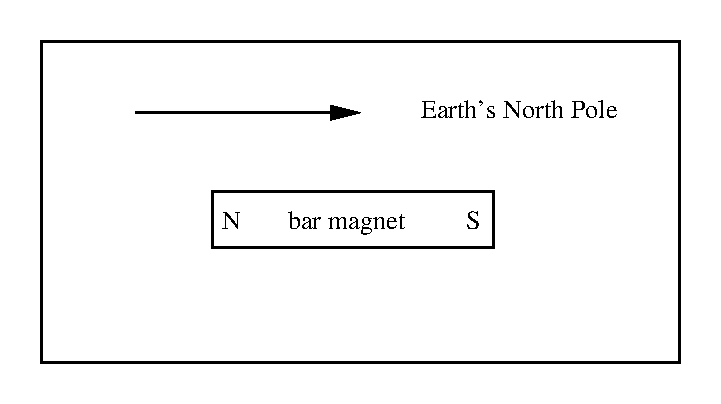
\includegraphics{magnetism_field_perm_mag/magnetism_2_fig_1.eps}} \par}
\vspace{0.3cm}

\begin{enumerate}
\item Trace the outline of a bar magnet on a piece of paper.
% and orient it so that the magnet's south pole points to the earth's geographic
% north pole.
 Indicate the magnet's polarity on the outline.
\item Place the small compass on the side of the magnet near the north pole
 and make a dot at each end of the needle using a pencil not encased in metal.
\item Move the compass forward until its south pole points at the previous
north pole dot, and make a new dot at the north pole (kind of a leap-frog 
effect).
\item Repeat 3 until the series of dots reaches the side of the magnet near 
the south pole or the edge of the paper.
\item In a similar manner, trace enough lines to map the magnetic field
over the entire paper.
%\item There are two points, called neutral points, near each end of the
%magnet where the magnet's field and the earth's field are equal and
%opposite and so cancel. At these points, the compass will align in
%no particular direction. Try to locate these points by tracing very
%carefully the lines of force in the neighborhood of the poles.
\item Do lines of force ever cross?\vspace{15mm}

\item Where is the magnetic field strongest? Weakest? How do the field
lines indicate this? Does a field line represent a constant field
along its entire length?\vspace{15mm}

\item Do the lines intersect the magnet at a particular angle (like the
electric field lines near a conductor)?\vspace{15mm}
%What does this imply about
%the source of a magnetic field as opposed to the surface charge of
%a conductor as the source of an electric field? \vspace{15mm}

\end{enumerate}
\textbf{Activity 2: Two Bar Magnets--Unlike Poles Facing One Another}

\vspace{0.3cm}
{\centering \resizebox*{0.45\textwidth}{!}{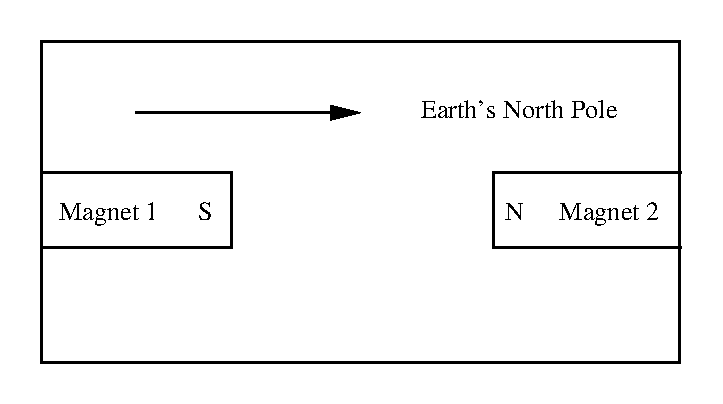
\includegraphics{magnetism_field_perm_mag/magnetism_2_fig_2.eps}} \par}
\vspace{0.3cm}

\begin{enumerate}
\item Set up two bar magnets on a sheet of paper as shown in the figure
above. The magnets should be 8-10 cm apart.
\item Repeat steps 2 through 5 from the previous activity.
\item What sort of charge configuration produces an electric field that
looks similar to the magnetic field you just identified?\vspace{30mm}

\item What differences can you recognize?\vspace{30mm}

\end{enumerate}

\newpage

\textbf{Activity 3: Two Bar Magnets--Like Poles Facing One Another}

\vspace{0.3cm}
{\centering \resizebox*{0.45\textwidth}{!}{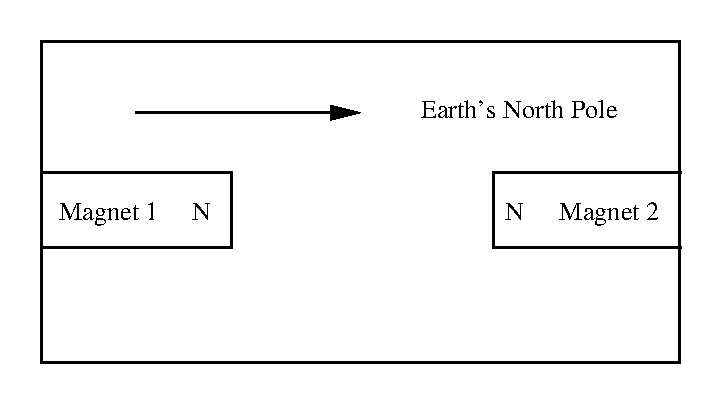
\includegraphics{magnetism_field_perm_mag/magnetism_2_fig_3.eps}} \par}
\vspace{0.3cm}

\begin{enumerate}
\item Set up two bar magnets on a sheet of paper as shown in the figure
above. The magnets should be 8-10 cm apart.
\item Repeat steps 2 through 5 from Activity 1 of this investigation.
\item Try to identify on your map a point at which the magnetic field is
zero. Explain what causes this effect.\vspace{30mm}

\item What sort of electric charge configuration would produce a similar
field map?\vspace{15mm}
\end{enumerate}

